% Created 2016-12-17 Sat 16:57
\documentclass[10pt,conference,compsocconf]{IEEEtran}
\usepackage[utf8]{inputenc}
\usepackage[T1]{fontenc}
\usepackage{fixltx2e}
\usepackage{graphicx}
\usepackage{grffile}
\usepackage{longtable}
\usepackage{wrapfig}
\usepackage{rotating}
\usepackage[normalem]{ulem}
\usepackage{amsmath}
\usepackage{amssymb}
\usepackage{textcomp}
\usepackage{amssymb}
\usepackage{capt-of}
\usepackage{hyperref}
\usepackage{bm}
\usepackage{svg}
\usepackage{graphicx}
\graphicspath{{pics/}}
\usepackage[margin=1in]{geometry}
\usepackage{algorithm}
\usepackage{algpseudocode}
\graphicspath{{pics/}}

\def\arraystretch{1.7}
\author{Laurent Lejeune, Tatiana Fountoukidou, Guillaume de Montauzon}
\date{\today}
\title{Group 97: Road Segmentation}
\hypersetup{
	pdfauthor={Laurent Lejeune, Tatiana Fountoukidou, Guillaume de Montauzon},
	pdftitle={Group 97: Road Segmentation},
	pdfkeywords={},
	pdfsubject={},
	pdfcreator={Emacs 25.1.1 (Org mode 8.3.6)}, 
	pdflang={English}}
\begin{document}
	
	\maketitle
	
	\section{Introduction}

  The goal of this project is to classify roads in satellite images. 
	An example is shown in figure \ref{fig:example}. This report is structured as
  follows. We start from a baseline where basic features (mean and variance of
  RGB va lues) are extracted. Three classifiers are then used: Logistic
  regression, Support Vector Machine (SVM) using radial basis function kernel,
  and random forest. We then introduce a more elaborate attempt using a feature
  set made of Scale Invariant Feature Transform (SIFT) and Hough line transform
  among others. Generic classifiers similar to our baselines are then applied
  and their predictions are refined using a structured output model called
  structured SVM. A third attempt, by far the most effective, makes use of the Unet Convolution Neural Network.
  The next section gives the procedure and results of our baseline classification.
	\begin{figure}[h]
		\centering
		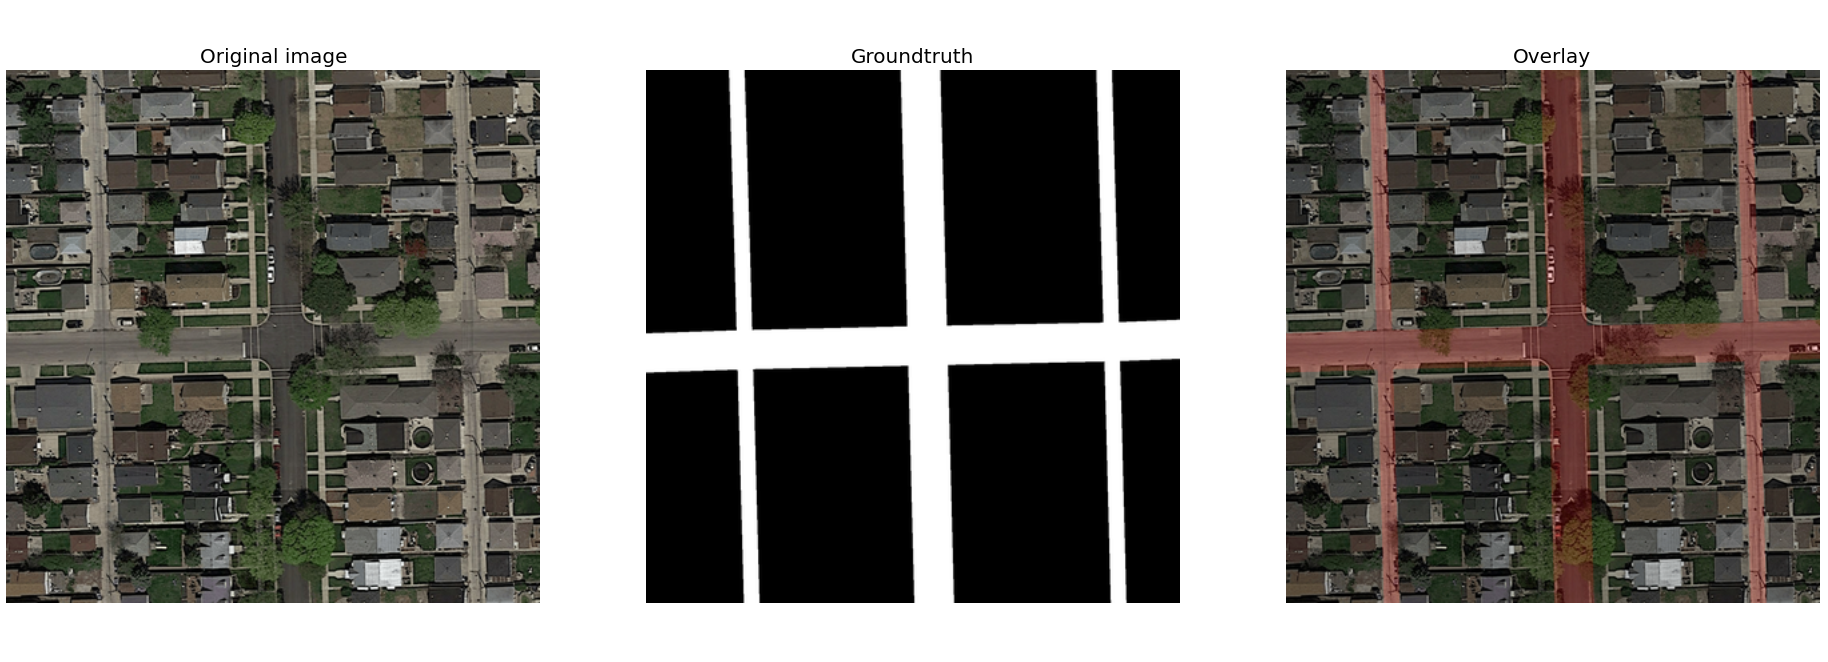
\includegraphics[width=0.5\textwidth]{pics/example.png}
		\caption{Example of training image with its ground-truth}
		\label{fig:example}
	\end{figure}
	
	\section{Data exploration}
	The provided training set contains 100 images of size 400x400 along with their
  ground-truth. A total of 6 images are discarded because they either show too few positive class pixels, or some misleading regions such as rail-tracks. 
	We notice that most images are made of grid-like roads, sometimes occluded by trees. 

	\section{Baselines}
	\subsection{Comparison of classifiers}
	\label{baseline_selection}

  The images are first cropped into non-overlapping square patches. As features,
  the mean and variance RGB values are extracted in each patch. As for the
  generation of ground-truth samples, a patch $p_i \in
  \left\{0;1\right\}^{d \times d}$ is
  considered a positive sample if $\frac{\sum_{j}{p_i}}{d^2} > 0.25$, and negative otherwise.
A grid search was performed on the hyper-parameters of three different classifiers:
  Logistic regression, SVM with RBF kernel, and random forest.
	The performance metric is the F1-score, which computes the
  harmonic mean of precision and recall.
	The scores and the optimal values of hyper-parameters are shown in table
  \ref{baseline}. Let us note that random forest is significantly faster to
  train than SVM. This drives our choice to discard the latter for the remaining
  of this work.
		\begin{table}[h]
		\caption{\label{baselines}Baselines}
		\centering
		\begin{tabular}{p{0.3\textwidth} c}		
			\textbf{Classifier} &  \textbf{$F_1-score (\text{mean}\pm \text{std})$}\\
			\hline \hline
			Logistic regression ($\lambda = 1e-2$) & $0.44 \pm 0.02$ \\ \hline
			SVM (rbf kernel, $\lambda = 1e5$) & $0.5 \pm 0.02$ \\ \hline
			\textbf{RF (number of trees = 50, max depth = 10)} & $\bf{0.5 \pm 0.02}$ \\
			\hline
		\end{tabular}
		\end{table}
	\subsection{Influence of patch size}
    Table \ref{patch_size} summarizes our baseline results.
	\begin{table}[h]	
	\centering
	\begin{tabular}{lc}
		\hline \hline		
		\textbf{Patch Size} &  \textbf{F-score (mean $\pm$ std)} \\
		\hline
		8 & $0.45 \pm 0.03$ \\
		16 & $0.5 \pm 0.03$ \\
		25 & $0.54 \pm 0.04$ \\
		32 & $0.55 \pm 0.06$ \\
		\hline
	\end{tabular}
	\caption{\label{patch_size}Patch size comparison}
	\end{table}
	Even though the larger the patch size, the better the F-score, we observed that many roads were too narrow to be represented by a larger patch size. The higher score in this case is misleading, since it is calculated on a patch level, and not on a pixel level. This way, although more patches are classified correctly, the overall segmentation mask that comes up is not representative enough. For this reason, the patch size of 16 was kept, as more appropriate to capture the different road widths.
For the rest of the work,
  the performance of the random forest (RF) classifier will be used as the
  baseline
	\section{Structured SVM approach}
  Prior to feature extraction, our images are pre-segmented using	SLIC
  Superpixels (Simple Linear Iterative Clustering) \cite{achanta12}, which
  groups pixels in mid-level regions in an iterative manner. The algorithm
  starts from a regular grid of cluster centers and iteratively updates the
  labels of their neighboring centers based on a distance measure. In comparison
  with square patches, superpixels allow to extract more discriminative regions.
  The next section describes the feature extraction and their encoding.
\subsection{Feature extraction}

\begin{figure}[htb]
\centering
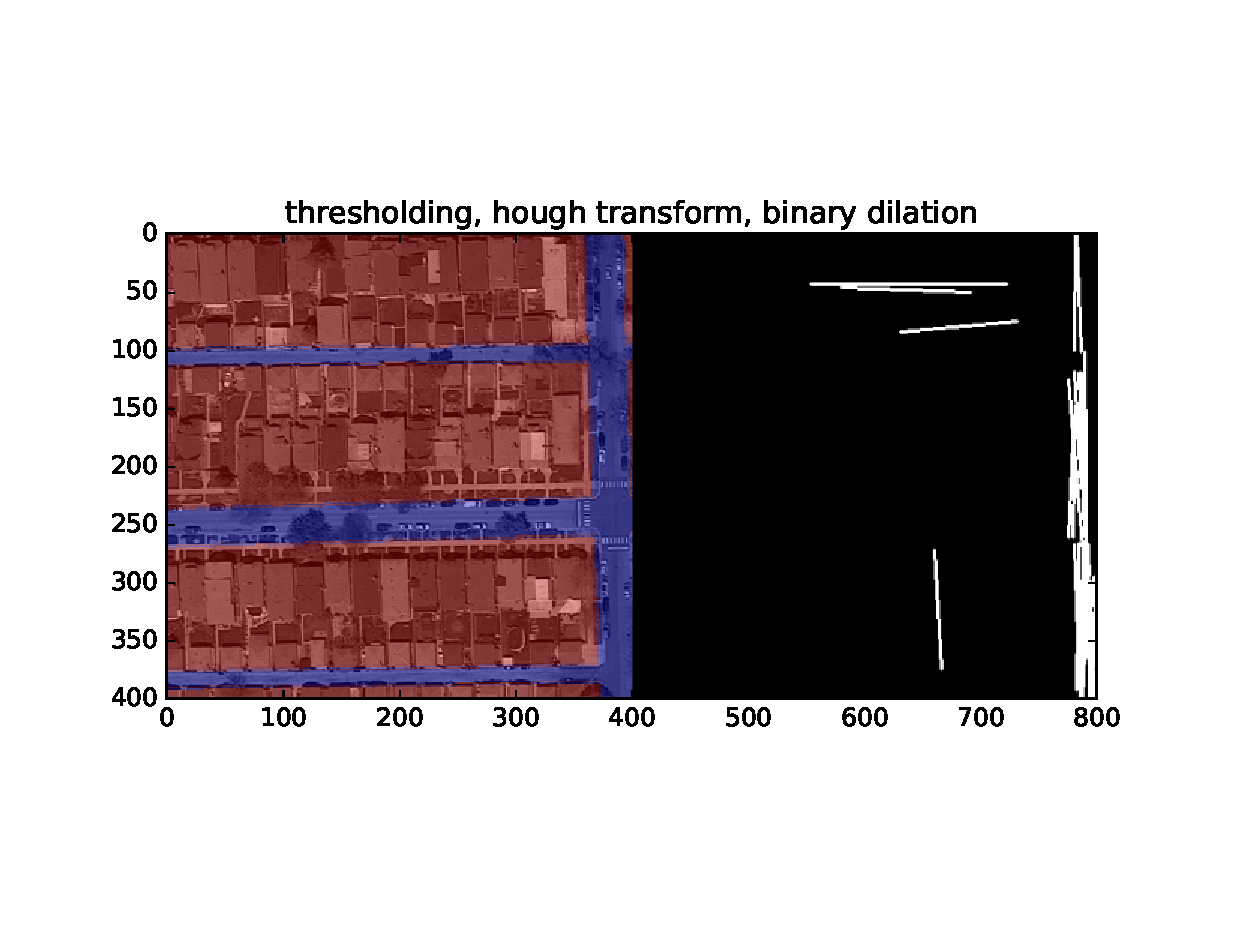
\includegraphics[width=0.5\textwidth]{pics/ex_hough.eps}
\caption{\label{fig:hough}
Example of a hough transform. Left: Input image with the ground-truth overlay. Right: 20 lines with lowest color variance.}
\end{figure}

Following an exploration of the related litterature, we select a set of features to extract.
\begin{itemize}
\item SIFT (Scale-Invariant Feature Transform) \cite{lowe04}: This descriptor is used extensively in computer-vision applications. It computes a histogram of oriented gradients on 16x16 windows centered at a keypoint and gives a descriptor of 128 scalar values. The keypoint detection step is not performed, instead we extract the descriptors on a dense grid at canonical scale and orientation. As advised in \footnote{\url{https://people.csail.mit.edu/hasinoff/320/sift-notes.txt}}
 to improve illumination invariance, the integer value descriptors are first normalized to unit-norm, ceiled to 0.2, and renormalized to unit-norm. As we require that each segment be represented by a single feature vector, we encode the dense SIFT descriptors contained in a given segment in a "bag-of-features" manner through the following steps: 
\begin{enumerate}
\item Based on a sufficiently large number of SIFT descriptors computed on 10 images, we start by fitting a PCA model. We have checked that the explained variance at 60 components is above 99\%.
\item A codebook is generated on the aforementioned training samples. A codebook is merely a set of K-means clusters that is used to encode the input (compressed) descriptors to integer values.
\item We then compute a normalized histogram of codes (bag-of-features) in each segment. This gives us a single texture feature vector for mid-level regions.
\end{enumerate}
\item Hough line transform: This transformation has already been used in a state-of-the-art method \cite{2016ISPAr41B3..891L}. First, the edge map is computed using a canny edge detector. Given some parameters, a set of lines are extracted on the edge maps and sorted based on their RGB variance, i.e. we want to keep the lines along which the color variations is minimal. An example is shown on figure \ref{fig:hough}. As feature, we take the mean value of the hough map on the segment.
\item Euclidean distance transform. This straightforward transform is used to compute, at each pixel location, the shortest "taxicab" distance to an edge pixel. Using as input the canny edge map, we expect this feature to discriminate cluttered regions such as those containing blocks of buildings where the Euclidean distance tends to be smaller. The mean value over the segment is used.
\item Mean RGB value. Roads tend to have greyish colors.
\end{itemize}
To summarize, our feature extraction procedure provides a total of 65 features
per superpixel.

\subsection{Refinement of generic models using structured SVM}
\begin{figure}[htb]
\centering
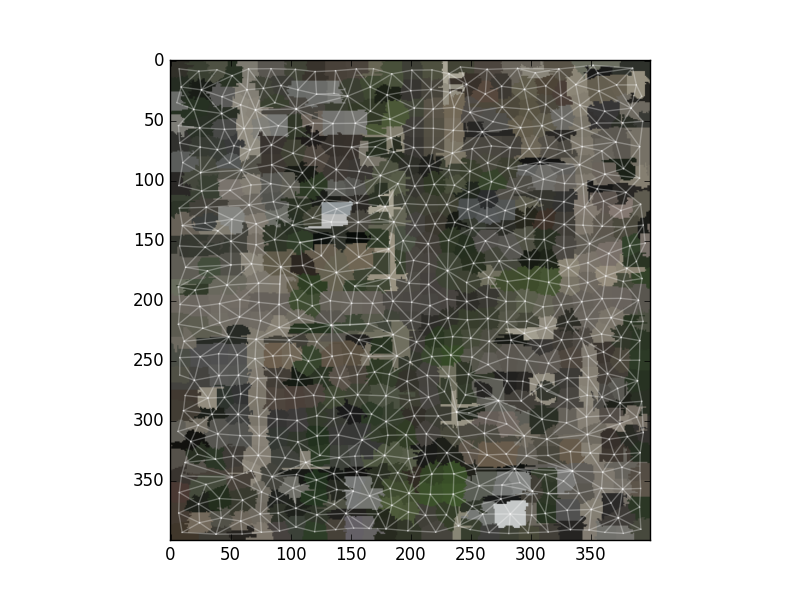
\includegraphics[width=0.4\textwidth]{pics/ex_graph.png}
\caption{\label{fig:graph}
Example of a superpixel-segmented image with connecting edges.}
\end{figure}

   Using structured models \cite{tsochantaridis05}, one can leverage the spatial
   relations between mid-level regions. As shown on figure \ref{fig:graph},a
   segment considered as road gives a strong prior on the "roadness" of its
   neighboring segment. This is formalized as an undirected graph on which the
   node features are assigned unary potentials. In our case, the unary
   potentials are given by probability estimates given by any generic models such as logistic regression or random forest.
Inspired by \cite{fulkerson09}, the edge costs are made off of two features: The difference in mean LUV color, and the number of pixels that separate two segments (length of separating path). This last feature allows to penalize segments that are "weakly" connected. Indeed, we have verified visually that roads tend to be composed of regular chains of square-like segments, thereby justifying that choice.

Formally, structured models aim at maximizing an energy functions of the form:

 \begin{equation}
 \begin{split}
E_w(X,Y) &= \sum_{i \in \mathcal{V}} E_{data}(y_i;x_i) + \sum_{i,j \in \mathcal{E}} E_{smooth}(y_i;y_j) \\
 &= \mathbf{w}^T \psi(X,Y)
 \end{split}
 \end{equation}

Where \(\mathcal{V}\) is the set of vertices representing a segment, \(\mathcal{E}\) are the edges. The data and smoothness term are combined in the joint-features vector \(\psi\). The variable \(y\) represents the structured labels. In our setup, any probabilistic regression model (logistic regression, random forest,\ldots{}) can be used for the data term. Following \cite{fulkerson09}, the pair-wise edges potentials are given by:

 \begin{equation}
\phi(c_i,c_j|s_i,s_j) = \frac{L(s_i,s_j)}{1+\lVert s_i - s_j \rVert}
 \end{equation}
Where \(c\) and \(s\) are the mean LUV-space colors. The function \(L\) expresses the length of the shared boundaries between two segments.
The provided code relies on the pyStruct package \cite{muller14}, which implements the cutting-plane algorithm proposed by Tsochantaridis et al \cite{tsochantaridis05}.
	\section{Classification}
	Two methods were implemented. The first consists of feature extraction and classification, with the features mentioned aboved. The second consists of training a convolutional neural network (CNN) that takes as input the image and outputs a segmentation mask. Both approaches are described below. 	
	
	\subsection{Classification based on feature vectors}
	The features described above were used to train a random forest ensemble classifier. A grid search to define the hyperparameters of the classifier was performed. The chosen parameters were the following:
	$$\text{Number of trees} = 50$$
	$$\text{Maximum tree depth} = 10$$
	The CRF refinement step was then performed.
	\subsection{U-net}
	A convolutional neural network designed for image segmentation was used, as
  described in \cite{unet}. U-net is a fully convolutional neural network,
  meaning that it consists exclusively on convolutional and pooling layers, and
  not fully connected layers in the end. As a result, the output of the network
  is not a class assignment for the input, but a feature map. In our case the
  output of the network is a segmentation mask for the input image. The
  structure of the network is shown in figure \ref{fig:unet_arch}.
		\begin{figure}[h]
			\centering
			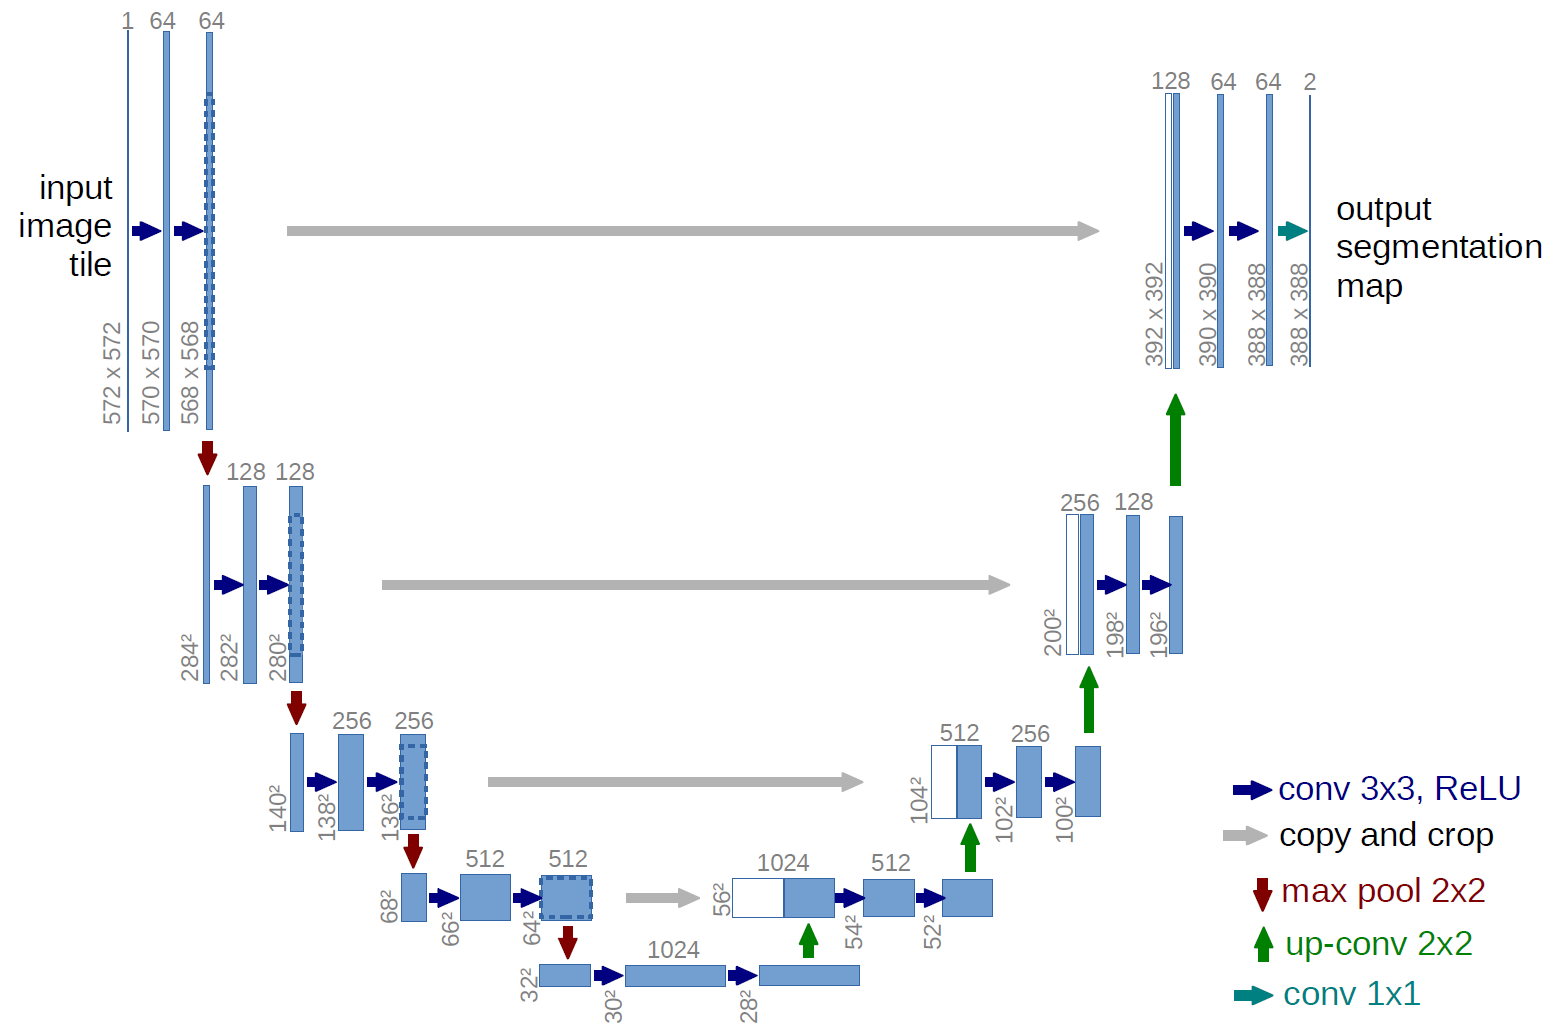
\includegraphics[width=0.5\textwidth]{pics/unet.png}
			\caption{U-net~\cite{unet}}
			\label{fig:unet_arch}
		\end{figure}
	\section{Results}
		\begin{table}
		\begin{tabular}{p{0.3\textwidth} c}		
			\textbf{Classification method} &  \textbf{$F_1-score (\text{mean}\pm \text{std})$}\\
			\hline \hline
			 Random forest, square patches, basic features [Baseline] & $0.5 \pm 0.02$ \\ \hline
			Logistic regression ($\lambda = 1e-2$), elaborate features& $0.45 \pm 0.02$ \\ \hline
			Random forest (50 trees, max. depth 10), elaborate features& $0.68 \pm 0.03$ \\ \hline
			Random forest, SSVM refinement, elaborate features & $0.79 \pm 0.02$ \\ \hline
			Logistic regression, SSVM refinement, elaborate features& $0.68 \pm 0.02$ \\ \hline
			U-net & $ $ \\
			\hline
		\end{tabular}
		\caption{\label{table:results}Concentrated results}
		\end{table}
	The results of a 5-fold cross validation, for the different classification
  approaches that were attempted and described above are shown in table \ref{table:results}
	\begin{figure}[h]
		\centering
		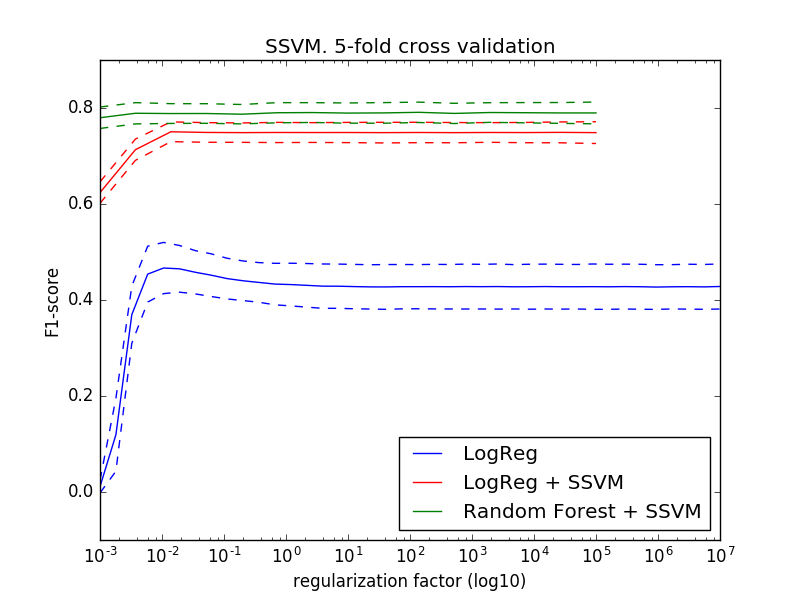
\includegraphics[width=0.5\textwidth]{pics/cross_val_ssvm.png}
		\caption{5-fold cross-validation using logistic regression, SSVM-refined
      logistic regression and SSVM-refined random forest}
		\label{fig:example}
	\end{figure}
		\begin{figure}[h]
			\centering
			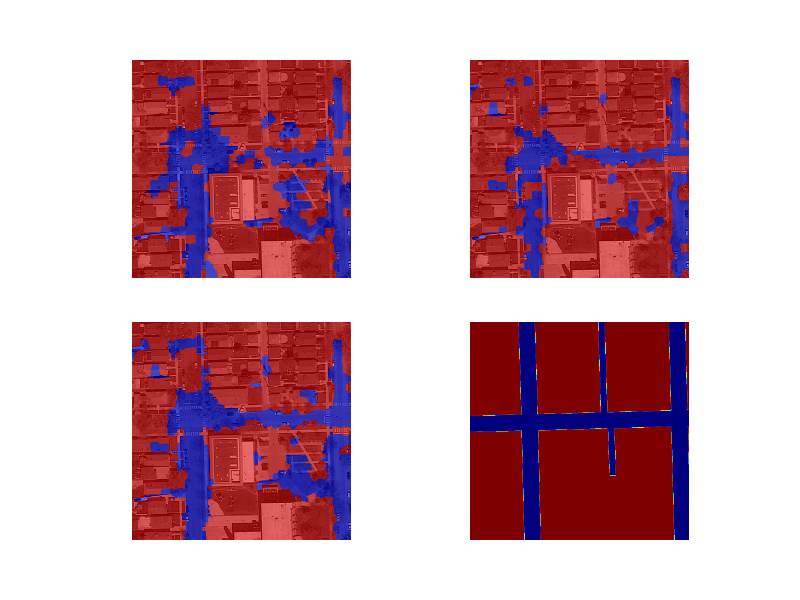
\includegraphics[width=0.5\textwidth]{pics/prediction.png}
			\caption{Example of prediction on unseen image. Top left: Logistic
        regression. Top right: Random forest. Bottom left: Refined random
        forest. Bottom right: Ground-truth.}
			\label{fig:predictions}
		\end{figure}
	\section{Conclusions}
	
	\bibliographystyle{ieeetr}
	\bibliography{refs}
	%\printbibliography
\end{document}